% =====================================================================
% Template Laporan Tugas — Workshop Deep Learning (Teknik Telekomunikasi ITERA)
% Studi Ablasi RNN, LSTM, GRU vs ANN untuk Prediksi Trafik Seluler
%
% Format IEEE conference dua kolom.
% Compile: pdflatex main && bibtex main && pdflatex main && pdflatex main
% =====================================================================
\documentclass[conference,a4paper]{IEEEtran}
\IEEEoverridecommandlockouts

\usepackage[indonesian]{babel}
\usepackage[utf8]{inputenc}
\usepackage[T1]{fontenc}
\usepackage{cite}
\usepackage{amsmath,amssymb}
\usepackage{graphicx}
\usepackage{booktabs}
\usepackage{siunitx}
\usepackage{xcolor}
\usepackage{multirow}
\usepackage[hidelinks]{hyperref}
\graphicspath{{gambar/}}

\begin{document}

\title{Studi Ablasi RNN, LSTM, dan GRU dibandingkan ANN untuk Prediksi Trafik Seluler Kota Milan}

\author{
\IEEEauthorblockN{Adif Dafa Raihan}
\IEEEauthorblockA{NIM 124400055\\
Teknik Telekomunikasi, ITERA\\
adif.124400055@student.itera.ac.id}
\and
\IEEEauthorblockN{Cindy Auliya}
\IEEEauthorblockA{NIM 124400045\\
Teknik Telekomunikasi, ITERA\\
cindy.124400045@student.itera.ac.id}
\and
\IEEEauthorblockN{Bima Cahya Ramadhan}
\IEEEauthorblockA{NIM 124400001\\
Teknik Telekomunikasi, ITERA\\
bima.124400001@student.itera.ac.id}
}

\maketitle

\begin{abstract}
Pertumbuhan trafik internet seluler menuntut operator meramalkan beban setiap sel secara akurat agar kapasitas dan energi jaringan dialokasikan secara efisien. Penelitian ini membandingkan ANN dengan RNN, LSTM, dan GRU untuk prediksi trafik per jam pada dataset Telecom Italia Big Data Challenge di Milan, dengan lokasi utama Duomo (kotak 5060) dan uji generalisasi di Navigli (kotak 4555). Kami melakukan studi ablasi terkontrol dengan mengubah satu faktor setiap kali, yaitu panjang jendela, ukuran hidden, jumlah lapisan, learning rate, kelompok fitur, dropout, dan horizon, masing-masing dengan tiga random seed. Konfigurasi dipilih hanya berdasarkan val MAE, lalu diuji pada minggu test dan periode Natal. Pada konfigurasi acuan, RNN memberikan test MAE terbaik ($229.6 \pm 5.1$) dan mengungguli baseline naif minggu lalu ($467.6$), sedangkan ANN terlemah di antara empat model ($309.9 \pm 5.9$). Penyetelan menurunkan MAE RNN menjadi $224.5$ dan LSTM dari $273.6$ menjadi $225.3$, tetapi konfigurasi terbaik GRU justru memburuk ($239.7$ versus $237.2$) karena overfit. Di Navigli urutan berubah dan ANN menjadi terbaik ($191.1 \pm 1.9$). Hasil ini menunjukkan bahwa keunggulan model sekuensial bergantung pada lokasi dan bahwa pemilihan hyperparameter berbasis validasi tidak selalu menjamin perbaikan pada data uji.
\end{abstract}

\begin{IEEEkeywords}
prediksi trafik seluler, RNN, LSTM, GRU, studi ablasi
\end{IEEEkeywords}

% ---------------------------------------------------------------------
\section{Pendahuluan}

Pertumbuhan trafik data seluler menuntut operator meramalkan permintaan tiap sel secara akurat untuk alokasi kapasitas, efisiensi energi, dan kualitas layanan. Peramalan yang terlalu rendah menyebabkan kongesti, sedangkan peramalan yang terlalu tinggi membuang kapasitas. Karena trafik mengikuti ritme harian, mingguan, dan karakter kawasan, model perlu menangkap dependensi temporal, bukan hanya hubungan antarfitur pada satu waktu.

ANN meratakan jendela observasi sehingga urutan waktu hilang. \textit{Recurrent neural network} (RNN) mempertahankan \textit{hidden state}, tetapi rentan terhadap \textit{vanishing gradient}. \textit{Long short-term memory} (LSTM) menambahkan gerbang input, forget, dan output serta \textit{cell state} \cite{hochreiter1997lstm}, sedangkan \textit{gated recurrent unit} (GRU) menyederhanakannya menjadi gerbang reset dan update \cite{cho2014gru}. Keunggulan model sekuensial tidak otomatis karena bergantung pada panjang jendela, kapasitas hidden, kedalaman, \textit{learning rate}, fitur, regularisasi, dan horizon. Studi ablasi yang mengubah satu faktor setiap kali memisahkan pengaruh faktor tersebut dari variasi antar-seed.

Kontribusi laporan ini ada tiga. Pertama, ablasi terkontrol lima faktor utama (panjang jendela, ukuran hidden, jumlah lapisan, \textit{learning rate}, kelompok fitur) dan dua faktor tambahan (dropout, horizon) pada empat model dengan tiga seed di Duomo. Kedua, pemilihan konfigurasi hanya dari val MAE, lalu evaluasi pada minggu test dan Natal bersama baseline naif. Ketiga, uji generalisasi konfigurasi acuan dan terbaik di Navigli (kotak 4555, kode 1).

% ---------------------------------------------------------------------
\section{Data dan Metode}

\subsection{Dataset}

Data berasal dari Telecom Italia Big Data Challenge \cite{barlacchi2015milan} yang mencakup aktivitas jaringan di Kota Milan, Italia. Kami memakai versi agregasi per jam \cite{zhang2021fedda} untuk periode 4 November--29 Desember 2013, sehingga setiap lokasi memiliki 1.344 observasi atau 56 hari. Setiap catatan memuat tiga kanal trafik, yaitu internet (\textit{net}), panggilan (\textit{call}), dan SMS (\textit{sms}). Fitur masukan berjumlah tujuh: net, call, sms, serta empat fitur waktu berupa sinus dan kosinus jam (\textit{jam\_sin}, \textit{jam\_cos}) dan hari (\textit{hari\_sin}, \textit{hari\_cos}). Fitur waktu merepresentasikan periodisitas sirkadian dan mingguan secara kontinu. Target peramalan adalah net satu jam ke depan.

Lokasi utama penelitian adalah kotak Duomo 5060 yang mewakili pusat aktivitas kota. Sebagai uji generalisasi, kami memakai lokasi kelompok, yaitu Navigli (Darsena) pada kotak 4555 dengan kode lokasi 1. Sebaran kedua lokasi ditunjukkan pada Gambar~\ref{fig:peta}.

\begin{figure}[t]
  \centering
  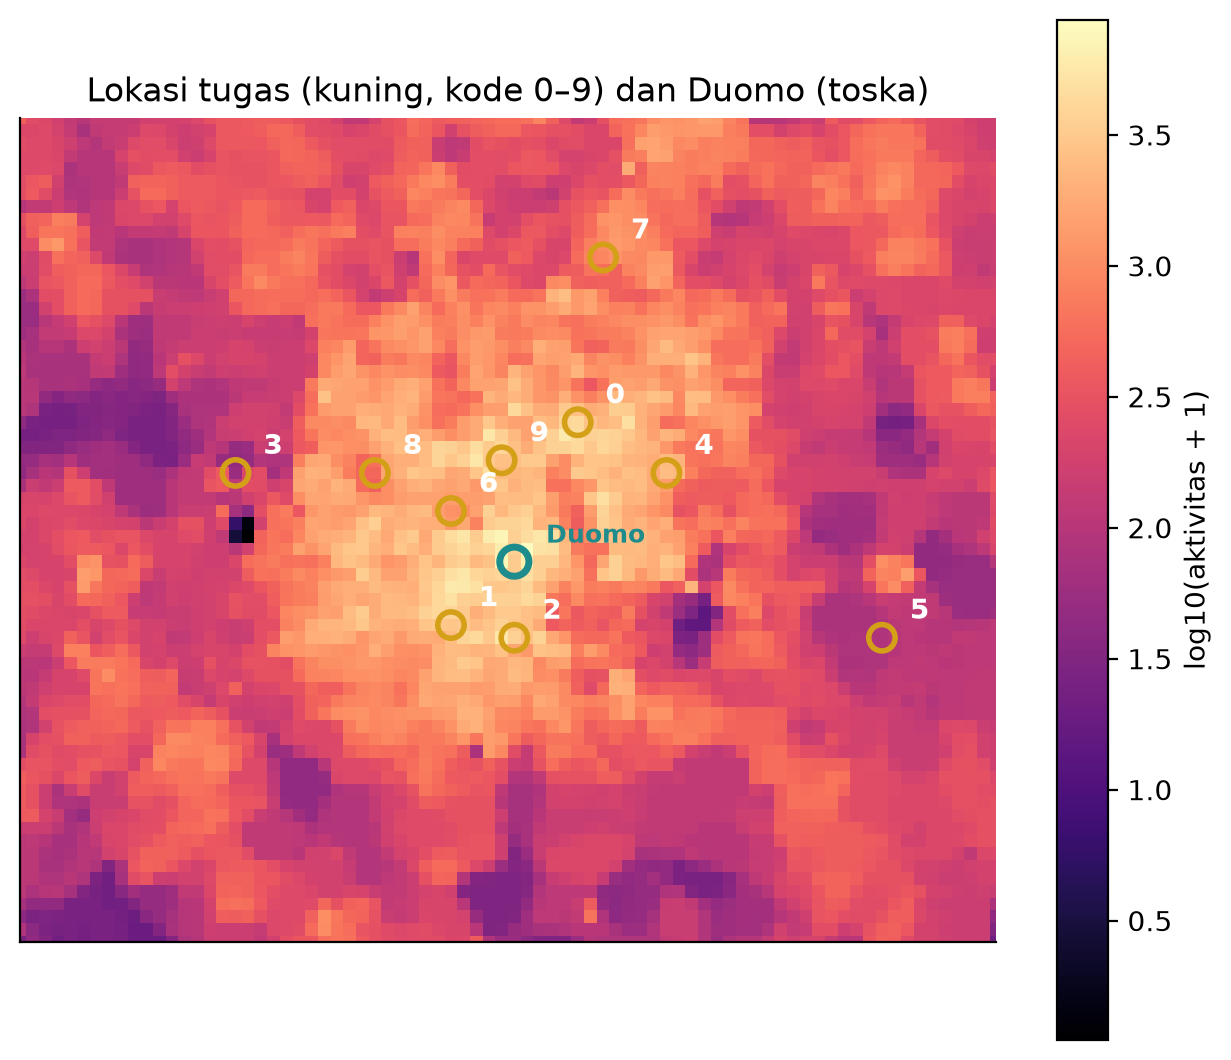
\includegraphics[width=0.85\linewidth]{peta_lokasi_tugas.png}
  \caption{Rata-rata aktivitas internet per kotak di Milan. Lingkaran kuning menunjukkan lokasi tugas (kode 0--9); lingkaran toska menunjukkan Duomo.}
  \label{fig:peta}
\end{figure}

\subsection{Pembagian Data dan Praproses}

Pembagian data dilakukan secara kronologis: train 11 November--8 Desember 2013 (672 jam), validasi 9--15 Desember, test 16--22 Desember, dan periode Natal 23--29 Desember. Minggu pertama, 4--10 November, tidak dipakai sebagai sampel latih dan hanya menjadi konteks jendela bagi sampel awal. Pembagian ini memisahkan masa depan dari masa lalu sehingga tidak ada informasi test yang bocor ke pelatihan.

Standardisasi z-score dihitung dari rata-rata dan simpangan baku data sebelum 9 Desember, yaitu data latih beserta minggu konteks. Statistik tersebut kemudian diterapkan pada validasi, test, dan Natal. Dengan cara ini, model tidak pernah melihat statistik periode evaluasi. Jendela masukan dibentuk dengan panjang $W = 24$ jam dan horizon $H = 1$ jam, sehingga terdapat 672 jendela latih. Sebuah jendela dimasukkan ke split tertentu berdasarkan waktu targetnya, bukan waktu awal jendela. Prediksi dikembalikan ke skala asli sebelum metrik dihitung.

Data deret waktu tidak diacak pada tahap pembagian karena pengacakan akan mencampur masa lalu dan masa depan serta merusak urutan yang menjadi objek peramalan. Pengacakan hanya dilakukan pada urutan \textit{mini-batch} selama pelatihan; setiap jendela tetap mempertahankan urutan internalnya.

\subsection{Model dan Konfigurasi Acuan}

ANN meratakan jendela $W \times 7$ menjadi vektor dan memetakannya melalui dua lapisan tersembunyi berukuran 32 dengan aktivasi ReLU. Model ini tidak memodelkan urutan secara eksplisit. RNN sederhana memproses jendela langkah demi langkah dengan \textit{hidden state} berukuran 68 dan memakai state terakhir untuk prediksi. LSTM memakai \textit{hidden state} 33 serta tiga gerbang dan \textit{cell state} \cite{hochreiter1997lstm}, sedangkan GRU memakai \textit{hidden state} 38 dengan dua gerbang \cite{cho2014gru}. Pada ketiga model rekuren, keluaran diambil dari \textit{hidden state} langkah terakhir, lalu dilewatkan satu lapisan linear.

Semua model dilatih dengan fungsi loss MSE dan optimizer Adam (\textit{learning rate} $10^{-3}$), batch 64, serta \textit{early stopping} pada val MSE dengan \textit{patience} 30 dan maksimum 300 epoch. Bobot terbaik dipilih dari epoch dengan val MSE terendah. Pelatihan diimplementasikan dengan PyTorch \cite{paszke2019pytorch}. Konfigurasi acuan dirangkum pada Tabel~\ref{tab:acuan}.

\begin{table}[t]
  \centering
  \caption{Konfigurasi acuan dan jumlah parameter}
  \label{tab:acuan}
  \begin{tabular}{@{}ll@{}}
    \toprule
    Hyperparameter & Nilai acuan \\
    \midrule
    Panjang jendela $W$ & 24 jam \\
    Horizon & 1 jam \\
    Ukuran hidden & ANN 32, RNN 68, LSTM 33, GRU 38 \\
    Jumlah lapisan & ANN 2, rekuren 1 \\
    Fitur & net, call, sms, jam (sin/cos), hari (sin/cos) --- 7 fitur \\
    Jumlah parameter & ANN 6.497, RNN 5.305, LSTM 5.578, GRU 5.397 \\
    Optimizer, \textit{learning rate} & Adam, $10^{-3}$ \\
    \textit{Batch size} & 64 \\
    \textit{Early stopping} & \textit{patience} 30, maks.\ 300 epoch \\
    \bottomrule
  \end{tabular}
\end{table}

\subsection{Protokol Ablasi dan Evaluasi}

Setiap eksperimen mengubah satu faktor dari konfigurasi acuan, sedangkan faktor lain dipertahankan. Faktor A1 menguji panjang jendela $W \in \{6, 12, 24, 48, 168\}$ jam; A2 ukuran hidden $\{16, 32, 64, 128\}$; A3 jumlah lapisan $\{1, 2, 3\}$; A4 \textit{learning rate} $\{10^{-4}, 10^{-3}, 10^{-2}\}$; dan A5 kelompok fitur \{net, net+call+sms, net+waktu, semua\}. Dua faktor tambahan adalah B2 dropout $\{0; 0,2; 0,5\}$ dan B6 horizon $\{1, 6, 24\}$ jam. Setiap konfigurasi dilatih dengan tiga \textit{random seed}, yaitu 0, 1, dan 2, lalu dilaporkan sebagai rata-rata $\pm$ simpangan baku.

Evaluasi memakai MAE, RMSE, dan MAPE pada skala asli. MAE menjadi metrik utama karena satuannya sama dengan aktivitas trafik, sedangkan MAPE memberi gambaran error relatif. Pemilihan konfigurasi terbaik hanya memakai val MAE; data test dan Natal tidak dipakai sampai evaluasi akhir. Konfigurasi terbaik tiap model kemudian digabungkan pada Bagian C dan diuji generalisasinya pada Bagian D.

Seluruh pelatihan dijalankan pada CPU dengan PyTorch. Sebanyak 270 pelatihan unik (348 catatan run karena beberapa konfigurasi acuan dipakai ulang) memerlukan total waktu 92,6 menit.

% ---------------------------------------------------------------------
\section{Hasil}

\subsection{Baseline Naif dan Acuan}

Evaluasi diawali dengan membandingkan performa model \textit{deep learning} pada konfigurasi acuan terhadap tiga metode \textit{baseline} naif tanpa parameter di lokasi Duomo (kotak 5060) dengan horizon peramalan satu jam ($H = 1$). Tiga \textit{baseline} naif yang diuji mencakup: (1) \textit{naif nilai terakhir} ($\hat{y}_t = y_{t-1}$), (2) \textit{naif kemarin} ($\hat{y}_t = y_{t-24}$), dan (3) \textit{naif minggu lalu} ($\hat{y}_t = y_{t-168}$). Hasil komparasi disajikan pada Tabel~\ref{tab:baseline_acuan}.

\begin{table}[t]
  \centering
  \caption{Baseline Naif dan Konfigurasi Acuan di Duomo ($H=1$, rata-rata $\pm$ SD, 3 seed)}
  \label{tab:baseline_acuan}
  \begin{tabular}{@{}lccccc@{}}
    \toprule
    Metode / Model & Param & Val MAE & Test MAE & Test MAPE (\%) & Natal MAE \\
    \midrule
    Naif: nilai terakhir & 0 & $662.6$ & $600.9$ & $18.4\%$ & $431.2$ \\
    Naif: kemarin & 0 & $595.3$ & $552.2$ & $23.8\%$ & $921.5$ \\
    Naif: minggu lalu & 0 & $492.8$ & $467.6$ & $19.9\%$ & $1426.2$ \\
    \midrule
    \textbf{ANN} (Acuan) & 6,497 & $248.9 \pm 8.9$ & $309.9 \pm 5.9$ & $11.3 \pm 0.8\%$ & $680.1 \pm 52.0$ \\
    \textbf{RNN} (Acuan) & 5,305 & $206.1 \pm 7.4$ & $229.6 \pm 5.1$ & $8.5 \pm 0.3\%$ & $421.2 \pm 2.4$ \\
    \textbf{LSTM} (Acuan) & 5,578 & $230.5 \pm 12.2$ & $273.6 \pm 25.4$ & $9.1 \pm 1.0\%$ & $586.0 \pm 56.8$ \\
    \textbf{GRU} (Acuan) & 5,397 & $207.5 \pm 3.8$ & $237.2 \pm 9.3$ & $8.0 \pm 0.7\%$ & $468.2 \pm 21.8$ \\
    \bottomrule
  \end{tabular}
\end{table}

Pada minggu uji reguler (16--22 Desember 2013), metode naif minggu lalu menjadi acuan nirparameter terkuat dengan test MAE $467.6$, mengonfirmasi kuatnya musiman 7 hari di Duomo. Seluruh model \textit{deep learning} mengungguli \textit{baseline} naif secara signifikan: ANN menurunkan test MAE menjadi $309.9 \pm 5.9$ (turun 33,7\%), LSTM ke $273.6 \pm 25.4$ (turun 41,5\%), GRU ke $237.2 \pm 9.3$ (turun 49,3\%), dan Simple RNN mencatatkan kesalahan terendah $229.6 \pm 5.1$ (turun 50,9\%). Keunggulan model rekuren membuktikan pentingnya pengolahan temporal sekuensial dibanding perataan dimensi waktu pada ANN.

Pada metrik MAPE, seluruh model memangkas kesalahan relatif ke kisaran 8,0\%--11,3\% (naif berkisar 18,4\%--23,8\%). GRU mencatat MAPE terbaik ($8.0 \pm 0.7\%$) yang menegaskan efektivitas gerbang \textit{reset} dan \textit{update} menjaga kestabilan proporsi kesalahan di seluruh rentang magnitudo beban.

Pada minggu Natal (23--29 Desember 2013), anomali liburan menyebabkan lonjakan drastis pada \textit{baseline} musiman: naif minggu lalu melonjak tajam ke MAE $1426.2$ (MAPE 96,8\%) akibat memproyeksikan hari kerja normal ke masa libur. Sebaliknya, naif nilai terakhir membaik ke $431.2$ karena dinamika trafik berada pada tingkat rendah yang datar. Di antara model teruji, Simple RNN memperlihatkan ketahanan generalisasi tertinggi dengan Natal MAE $421.2 \pm 2.4$, mengungguli seluruh model lainnya dan baseline naif. ANN mengalami degradasi paling berat ($680.1 \pm 52.0$) akibat bobot statis fitur kalender yang memaksakan keluaran hari kerja saat aktivitas perkantoran Duomo libur.

\subsection{Ablasi Wajib}

Pada bagian ini, dilakukan studi ablasi terkontrol menggunakan protokol \textit{one-factor-at-a-time} (OFAT). Setiap subbagian (A1 hingga A5) hanya memvariasikan tepat satu faktor hiperparameter secara terisolasi, sementara seluruh faktor lainnya dibekukan pada nilai konfigurasi acuan (Tabel~\ref{tab:acuan}). Seluruh eksperimen dijalankan secara independen dengan 3 \textit{random seed} (0, 1, 2) untuk memisahkan efek faktor arsitektural dari variasi stokastik inisialisasi bobot. Pemilihan konfigurasi terbaik didasarkan pada metrik \textit{validation} MAE guna mencegah kebocoran data uji.

\subsubsection{Panjang Jendela Observasi ($W$)}
Eksperimen A1 menguji pengaruh panjang konteks historis $W \in \{6, 12, 24, 48, 168\}$ jam. Hasil test MAE dirangkum pada Tabel~\ref{tab:tabel_A1_W} dan visualisasi pada Gambar~\ref{fig:ieee_col_A1_W}.

\begin{table}[t]
  \centering
  \caption{Pengaruh panjang jendela $W$ terhadap test MAE (rata-rata $\pm$ SD, 3 seed). Tebal = konfigurasi terpilih via val MAE.}
  \label{tab:tabel_A1_W}
  \begin{tabular}{@{}lcccc@{}}
    \toprule
    $W$ (jam) & ANN & RNN & LSTM & GRU \\
    \midrule
    6   & $\mathbf{269.4 \pm 16.8}$ & $228.6 \pm 5.4$  & $\mathbf{276.4 \pm 14.7}$ & $249.8 \pm 1.4$ \\
    12  & $308.8 \pm 11.6$          & $233.2 \pm 11.2$ & $302.7 \pm 17.4$          & $246.1 \pm 13.5$ \\
    24  & $309.9 \pm 5.9$           & $229.6 \pm 5.1$  & $273.6 \pm 25.4$          & $237.2 \pm 9.3$ \\
    48  & $333.1 \pm 20.2$          & $\mathbf{224.5 \pm 11.7}$ & $304.4 \pm 27.1$ & $\mathbf{237.1 \pm 10.6}$ \\
    168 & $402.0 \pm 12.5$          & $233.5 \pm 4.8$  & $292.8 \pm 20.0$          & $237.2 \pm 10.6$ \\
    \bottomrule
  \end{tabular}
\end{table}

\begin{figure}[t]
  \centering
  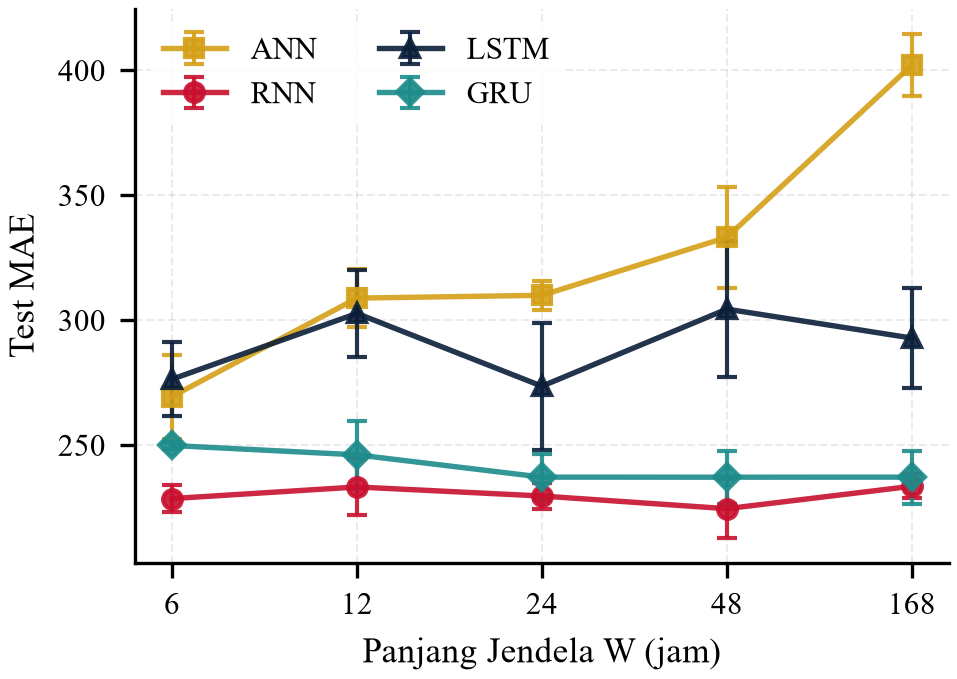
\includegraphics[width=0.9\linewidth]{ieee_col_A1_W.png}
  \caption{Test MAE terhadap panjang jendela $W$ untuk empat model di Duomo.}
  \label{fig:ieee_col_A1_W}
\end{figure}

Dari hasil eksperimen terungkap bahwa penambahan $W$ pada ANN memicu degradasi monotonik dari $269.4$ ($W=6$) ke $402.0$ ($W=168$) karena perataan matriks melipatgandakan parameter hingga 38.753, memicu \textit{curse of dimensionality}. Sebaliknya, model rekuren memiliki parameter konstan terhadap $W$ dan memperlihatkan ketahanan tinggi, dengan RNN dan GRU mencapai optimum validasi pada $W=48$ jam ($200.1 \pm 5.3$ dan $206.7 \pm 5.0$).

\subsubsection{Ukuran Lapisan Tersembunyi (\textit{Hidden Units})}
Eksperimen A2 mengevaluasi kapasitas representasi dengan memvariasikan dimensi hidden state $\in \{16, 32, 64, 128\}$ (Tabel~\ref{tab:tabel_A2_hidden}, Gambar~\ref{fig:ieee_col_A2_hidden}, dan Gambar~\ref{fig:ieee_col_A2_param}).

\begin{table}[t]
  \centering
  \caption{Pengaruh ukuran hidden terhadap val MAE (rata-rata $\pm$ SD, 3 seed)}
  \label{tab:tabel_A2_hidden}
  \begin{tabular}{@{}lcccc@{}}
    \toprule
    Hidden & ANN & RNN & LSTM & GRU \\
    \midrule
    16  & $257.6 \pm 28.0$ & $247.0 \pm 5.8$ & $244.3 \pm 18.3$ & $216.8 \pm 21.2$ \\
    32  & $248.9 \pm 8.9$ & $218.7 \pm 6.6$ & $241.5 \pm 20.5$ & $210.2 \pm 0.8$ \\
    64  & $238.4 \pm 16.5$ & $\mathbf{207.2 \pm 12.8}$ & $218.1 \pm 1.9$ & $198.4 \pm 9.2$ \\
    128 & $\mathbf{233.8 \pm 1.9}$ & $207.7 \pm 7.2$ & $\mathbf{207.1 \pm 8.4}$ & $\mathbf{188.7 \pm 4.2}$ \\
    \bottomrule
  \end{tabular}
\end{table}

\begin{figure}[t]
  \centering
  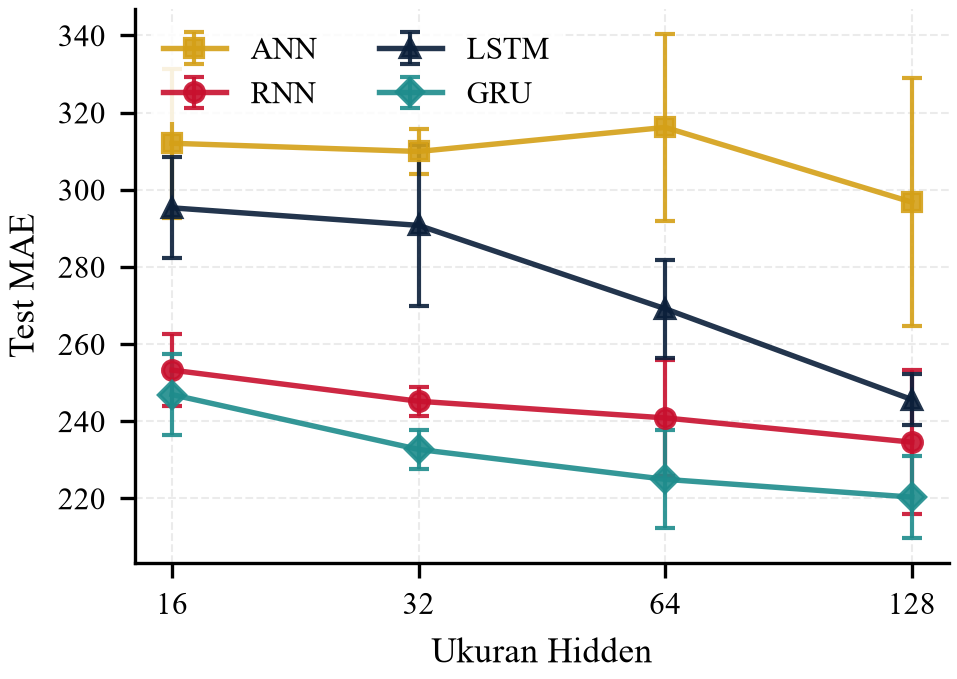
\includegraphics[width=0.9\linewidth]{ieee_col_A2_hidden.png}
  \caption{Test MAE terhadap ukuran hidden di Duomo.}
  \label{fig:ieee_col_A2_hidden}
\end{figure}

\begin{figure}[t]
  \centering
  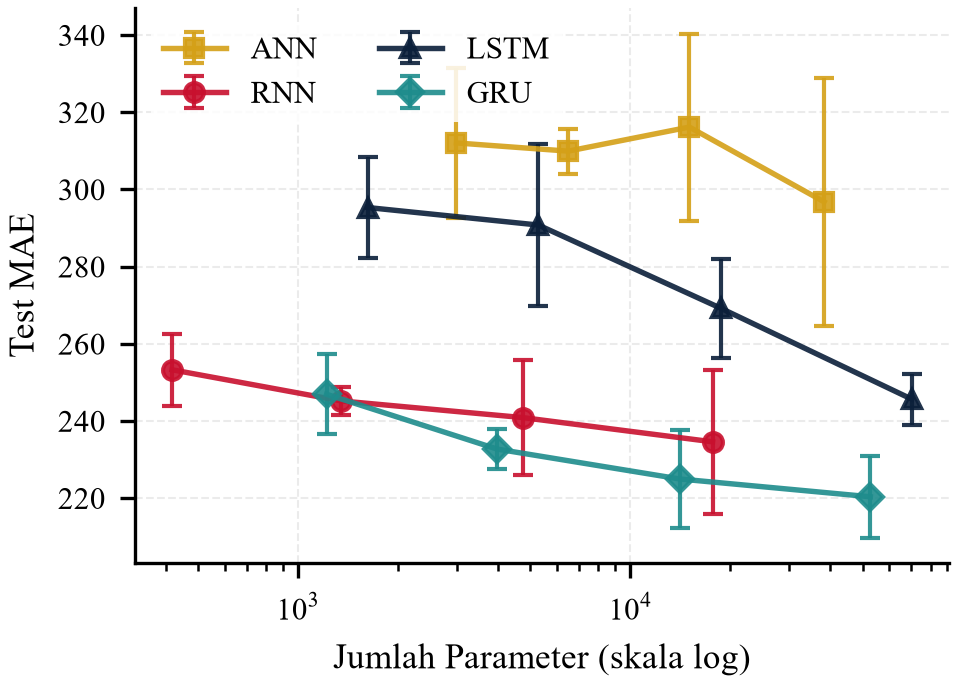
\includegraphics[width=0.9\linewidth]{ieee_col_A2_param.png}
  \caption{Jumlah parameter model terhadap ukuran hidden.}
  \label{fig:ieee_col_A2_param}
\end{figure}

Kapasitas rendah (16 unit) memicu \textit{underfitting} di seluruh model. Jumlah parameter rekuren berskala kuadratik terhadap hidden ($O(h^2)$): pada 128 unit, parameter LSTM melonjak ke 70.273, GRU ke 52.737, ANN ke 38.273, dan RNN ke 17.665. Kapasitas besar 128 unit secara konsisten menurunkan val MAE (GRU mencapai $188.7 \pm 4.2$ dan LSTM $207.1 \pm 8.4$), namun pertumbuhan parameter yang eksponensial menghadirkan \textit{diminishing returns} dan risiko \textit{overfitting}.

\subsubsection{Jumlah Lapisan}
Eksperimen A3 menguji kedalaman arsitektur dengan memvariasikan jumlah lapisan $\in \{1, 2, 3\}$ (Tabel~\ref{tab:tabel_A3_layers} dan Gambar~\ref{fig:ieee_col_A3_layers}).

\begin{table}[t]
  \centering
  \caption{Pengaruh jumlah lapisan terhadap val MAE (rata-rata $\pm$ SD, 3 seed)}
  \label{tab:tabel_A3_layers}
  \begin{tabular}{@{}lcccc@{}}
    \toprule
    Lapisan & ANN & RNN & LSTM & GRU \\
    \midrule
    1 & $\mathbf{240.9 \pm 7.5}$ & $\mathbf{206.1 \pm 7.4}$ & $\mathbf{230.5 \pm 12.2}$ & $207.5 \pm 3.8$ \\
    2 & $248.9 \pm 8.9$ & $207.3 \pm 9.1$ & $254.8 \pm 14.5$ & $\mathbf{203.3 \pm 9.6}$ \\
    3 & $244.9 \pm 5.4$ & $225.1 \pm 12.7$ & $338.9 \pm 16.9$ & $212.2 \pm 15.9$ \\
    \bottomrule
  \end{tabular}
\end{table}

\begin{figure}[t]
  \centering
  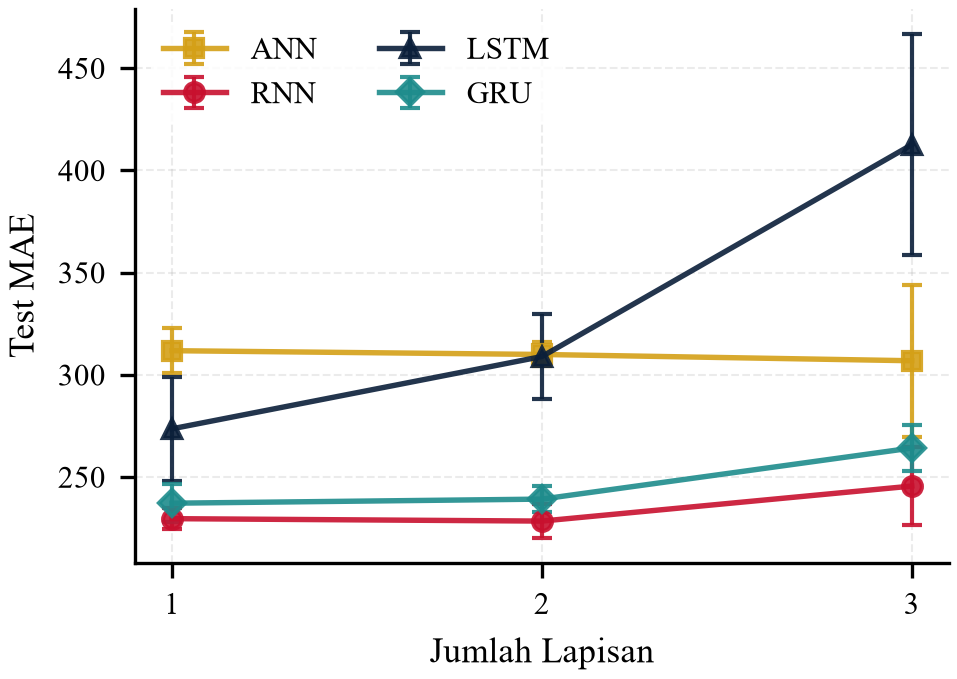
\includegraphics[width=0.9\linewidth]{ieee_col_A3_layers.png}
  \caption{Test MAE terhadap variasi jumlah lapisan.}
  \label{fig:ieee_col_A3_layers}
\end{figure}

Penambahan kedalaman ANN menghasilkan performa stabil ($240.9$ hingga $248.9$). Pada Simple RNN dan GRU, arsitektur dangkal 1--2 lapisan merupakan titik optimal. Sebaliknya, pada LSTM terjadi kegagalan katastropik saat diperdalam menjadi 3 lapisan: val MAE melonjak ekstrem dari $230.5$ (1 lapis) ke $338.9 \pm 16.9$ (3 lapis), dan test MAE anjlok ke $412.6$. Hal ini disebabkan oleh pelipatgandaan resistensi gradien (\textit{vanishing gradients}) saat melalui tiga lapis gerbang LSTM tanpa koneksi residual pada dataset berukuran kecil.

\subsubsection{Laju Pembelajaran (\textit{Learning Rate})}
Eksperimen A4 menguji $lr \in \{10^{-4}, 10^{-3}, 10^{-2}\}$ (Tabel~\ref{tab:tabel_A4_lr} dan Gambar~\ref{fig:ieee_col_A4_lr}).

\begin{table}[t]
  \centering
  \caption{Pengaruh learning rate terhadap val MAE (rata-rata $\pm$ SD, 3 seed)}
  \label{tab:tabel_A4_lr}
  \begin{tabular}{@{}lcccc@{}}
    \toprule
    Learning Rate & ANN & RNN & LSTM & GRU \\
    \midrule
    $10^{-4}$ & $295.3 \pm 4.6$ & $285.0 \pm 13.7$ & $399.4 \pm 25.0$ & $398.4 \pm 8.6$ \\
    $10^{-3}$ & $\mathbf{248.9 \pm 8.9}$ & $\mathbf{206.1 \pm 7.4}$ & $230.5 \pm 12.2$ & $\mathbf{207.5 \pm 3.8}$ \\
    $10^{-2}$ & $261.8 \pm 16.6$ & $226.7 \pm 6.7$ & $\mathbf{215.9 \pm 14.2}$ & $208.2 \pm 5.6$ \\
    \bottomrule
  \end{tabular}
\end{table}

\begin{figure}[t]
  \centering
  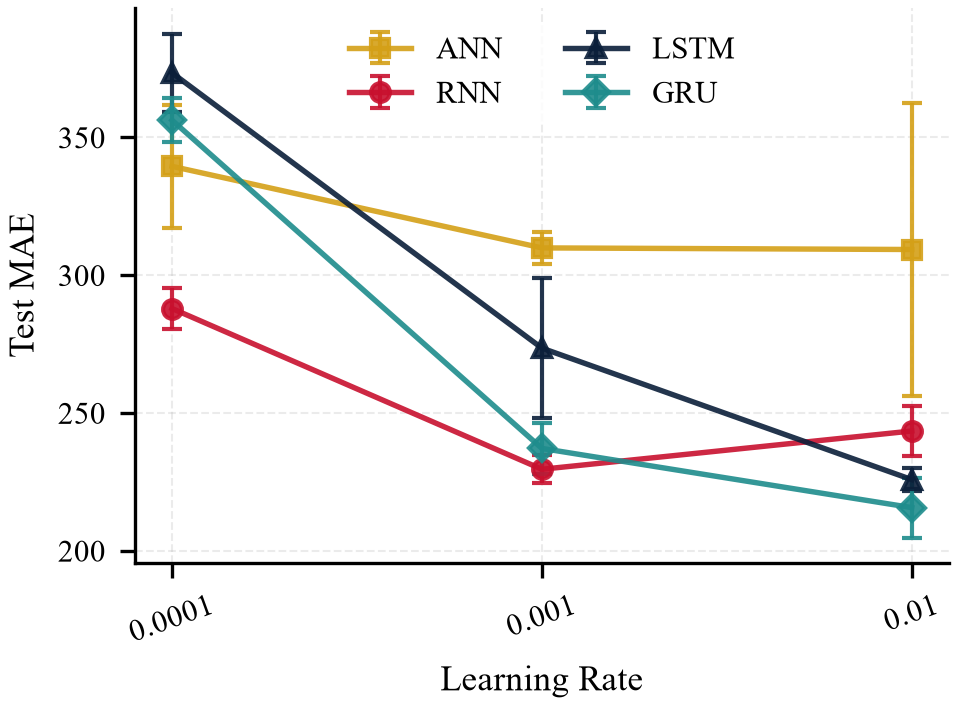
\includegraphics[width=0.9\linewidth]{ieee_col_A4_lr.png}
  \caption{Test MAE terhadap variasi learning rate.}
  \label{fig:ieee_col_A4_lr}
\end{figure}

Pada $lr=10^{-4}$, seluruh model menabrak batas 300 epoch tanpa memicu \textit{early stopping} (rata-rata epoch tepat 300.0) karena laju optimasi terlalu lambat, menyebabkan \textit{severe underfitting} (val MAE LSTM/GRU $\sim 399$). Laju $10^{-3}$ memberikan konvergensi stabil dan efisien bagi model sederhana (ANN, RNN, GRU). Sebaliknya, $10^{-2}$ mempercepat konvergensi (hanya 61--68 epoch) dan sangat menguntungkan arsitektur dengan gerbang non-linear (LSTM val MAE turun ke $\mathbf{215.9 \pm 14.2}$, test MAE $225.8$; GRU val MAE $208.2$, test MAE $215.7$), meskipun sedikit mendestabilisasi Simple RNN ($226.7$).

\subsubsection{Kelompok Fitur Masukan}
Eksperimen A5 memvariasikan komposisi fitur masukan: net saja, net+call+sms, net+waktu, dan semua fitur (Tabel~\ref{tab:tabel_A5_fitur} dan Gambar~\ref{fig:ieee_col_A5_fitur}).

\begin{table}[t]
  \centering
  \caption{Pengaruh kelompok fitur terhadap val MAE (rata-rata $\pm$ SD, 3 seed)}
  \label{tab:tabel_A5_fitur}
  \begin{tabular}{@{}lcccc@{}}
    \toprule
    Kelompok Fitur & ANN & RNN & LSTM & GRU \\
    \midrule
    net           & $260.5 \pm 7.0$          & $245.2 \pm 5.8$          & $266.2 \pm 5.7$          & $264.6 \pm 7.0$ \\
    net+call+sms  & $259.9 \pm 5.2$          & $224.1 \pm 2.3$          & $243.7 \pm 7.1$          & $231.8 \pm 12.6$ \\
    net+waktu     & $\mathbf{246.0 \pm 9.8}$ & $223.0 \pm 9.5$          & $231.1 \pm 4.3$          & $213.2 \pm 18.2$ \\
    semua         & $248.9 \pm 8.9$          & $\mathbf{206.1 \pm 7.4}$ & $\mathbf{230.5 \pm 12.2}$ & $\mathbf{207.5 \pm 3.8}$ \\
    \bottomrule
  \end{tabular}
\end{table}

\begin{figure}[t]
  \centering
  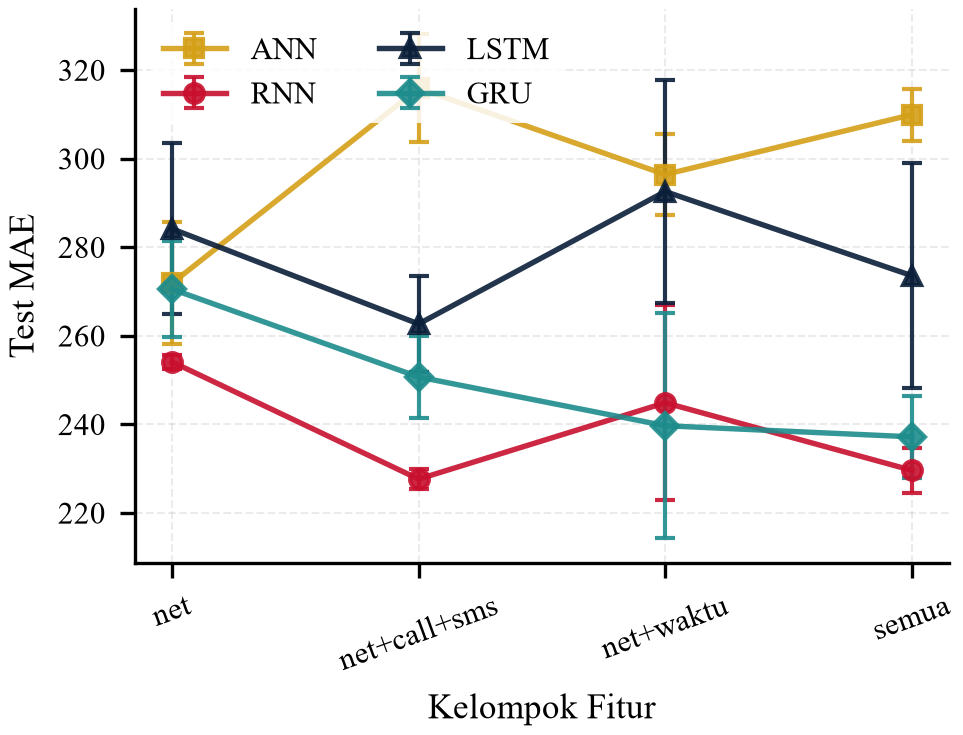
\includegraphics[width=0.9\linewidth]{ieee_col_A5_fitur.png}
  \caption{Test MAE untuk empat kelompok fitur di Duomo.}
  \label{fig:ieee_col_A5_fitur}
\end{figure}

Target univariat (net saja) menghasilkan val MAE tertinggi pada seluruh model rekuren ($>245$). Penambahan kanal panggilan dan SMS secara konsisten memangkas error rekuren (val MAE RNN turun dari 245.2 ke 224.1, LSTM dari 266.2 ke 243.7). Fitur waktu memberikan perbaikan validasi terbesar pada ANN ($246.0$) dan GRU ($213.2$). Kombinasi seluruh 7 fitur multimodal memberikan val MAE terbaik bagi model rekuren, membuktikan kemampuannya menyerap sinergi fitur tanpa meledakkan dimensi komputasi.

\subsection{Ablasi Pilihan}

Bagian ini menguji dua faktor lanjutan yang dipilih sebelum eksperimen dijalankan, yaitu dropout (B2) dan horizon peramalan (B6). Keduanya diuji pada empat model dengan 3 \textit{random seed}.

\subsubsection{B2. Dropout Rate}
\textbf{Hipotesis:} Dropout moderat ($p = 0.2$) meningkatkan generalisasi, sedangkan dropout agresif ($p = 0.5$) menyebabkan underfitting dan menaikkan error.

\begin{figure}[t]
  \centering
  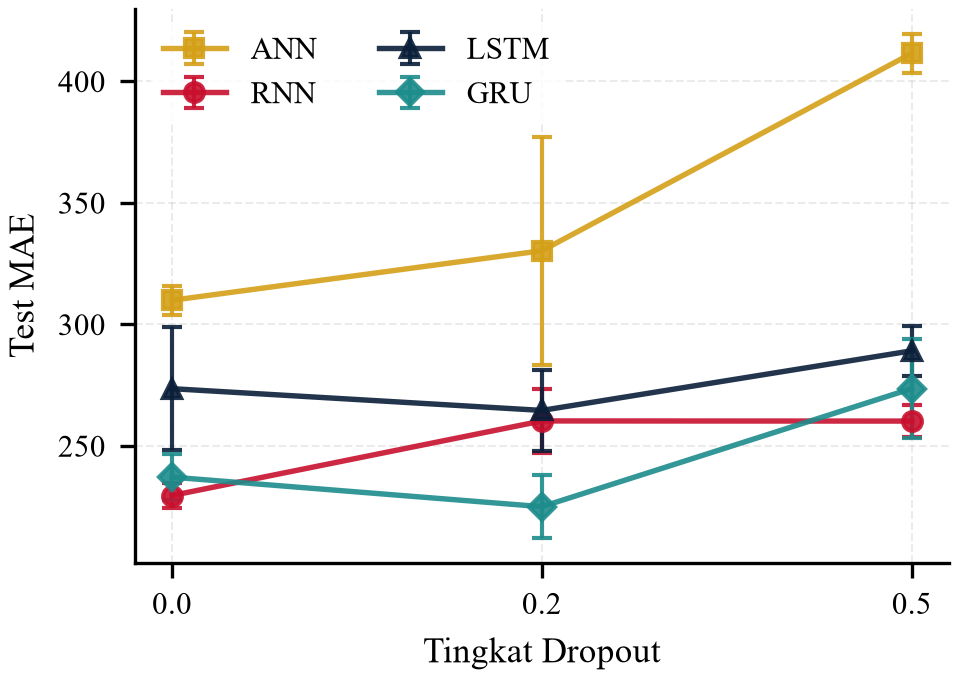
\includegraphics[width=0.9\linewidth]{ieee_col_B2_dropout.png}
  \caption{Test MAE terhadap tingkat dropout pada empat model di Duomo.}
  \label{fig:ieee_col_B2_dropout}
\end{figure}

\textbf{Hasil:} Dropout 0.2 menurunkan test MAE GRU dari $237.2$ ke $225.0$ (Natal membaik dari $468.2$ ke $429.7$) dan LSTM dari $273.6$ ke $264.6$. Val MAE GRU juga membaik dari $207.5$ ke $203.9$. Sebaliknya, ANN memburuk dari $309.9$ ke $330.3$ dan RNN dari $229.6$ ke $260.3$. Dropout agresif ($p = 0.5$) memicu underfitting parah pada seluruh model (test MAE ANN melonjak ke $411.6$, RNN ke $260.2$, LSTM ke $289.1$, dan GRU ke $273.6$).

\textbf{Status Hipotesis:} Sebagian didukung. Manfaat regularisasi moderat hanya berlaku bagi model bergerbang (terutama GRU); klaim universal tidak terbukti. Namun, hipotesis underfitting pada $p = 0.5$ terbukti penuh pada seluruh model.

\subsubsection{B6. Horizon Peramalan}
\textbf{Hipotesis:} MAE meningkat monoton seiring memanjangnya horizon ($H=1 < H=6 < H=24$). Pada $H=1$, neural network mengungguli baseline naif; pada $H=24$, keunggulannya mengecil dan model rekuren lebih unggul dibanding ANN.

\begin{figure}[t]
  \centering
  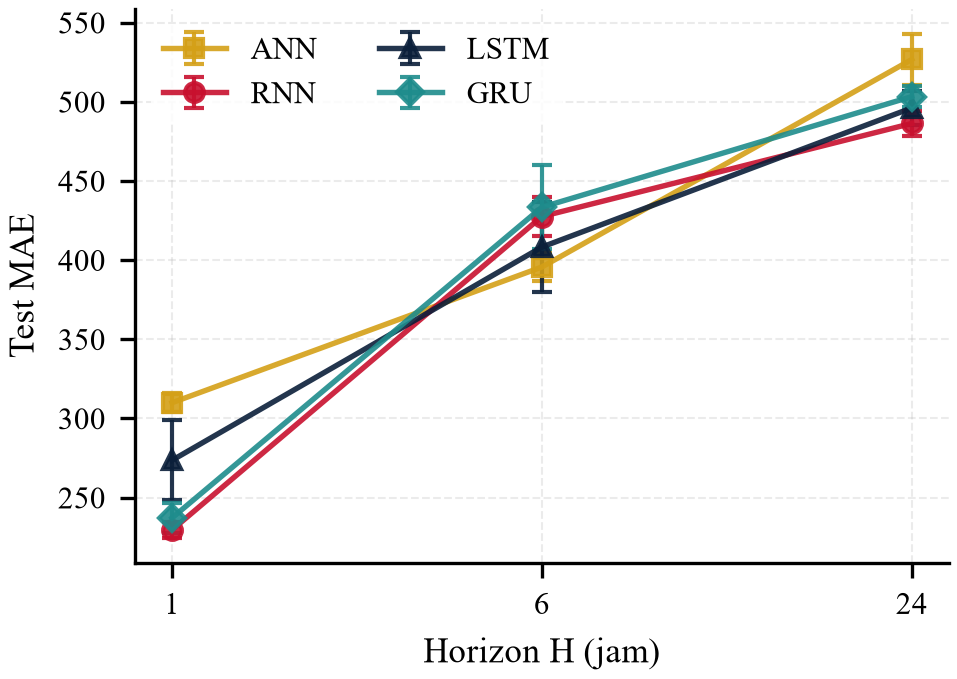
\includegraphics[width=0.9\linewidth]{ieee_col_B6_horizon.png}
  \caption{Test MAE terhadap horizon peramalan pada empat model di Duomo.}
  \label{fig:ieee_col_B6_horizon}
\end{figure}

\textbf{Hasil:} Test MAE meningkat secara monoton pada seluruh model. Pada $H=1$, model berkisar $229.6$--$309.9$, mengungguli baseline naif terbaik ($467.6$). Pada $H=6$, error naik ke kisaran $395.7$--$433.4$. Pada $H=24$, seluruh model menderita kenaikan ke rentang $486.4$--$526.8$ dan kalah dari baseline naif minggu lalu ($466.1$). Pada $H=24$, model rekuren (RNN $486.4$, LSTM $496.1$, GRU $503.3$) terbukti mengungguli ANN ($526.8$).

\textbf{Status Hipotesis:} Didukung sepenuhnya untuk monotonisitas dan penyusutan margin keunggulan pada peramalan multi-langkah.

\subsection{Bagian C — Konfigurasi Terbaik}

Berdasarkan hasil studi ablasi individual pada Bagian A dan B, konfigurasi terbaik tiap arsitektur dipilih murni berdasarkan metrik \textit{validation MAE} terendah (Tabel~\ref{tab:terbaik_duomo} dan Gambar~\ref{fig:ieee_col_C_terbaik_vs_acuan}). Horizon tetap dipertahankan pada $H = 1$ jam.

Kombinasi parameter terbaik terpilih:
\begin{itemize}
  \item \textbf{ANN Terbaik:} $W = 6$, hidden 128, 1 lapis, fitur \texttt{net+waktu} (4.097 param).
  \item \textbf{RNN Terbaik:} $W = 48$, hidden 68, 1 lapis, fitur \texttt{semua} (5.305 param).
  \item \textbf{LSTM Terbaik:} $W = 6$, hidden 128, 1 lapis, $lr = 10^{-2}$, fitur \texttt{semua} (70.273 param).
  \item \textbf{GRU Terbaik:} $W = 48$, hidden 128, 2 lapis, dropout 0.2, fitur \texttt{semua} (151.809 param).
\end{itemize}

\begin{table}[t]
  \centering
  \caption{Perbandingan Konfigurasi Acuan vs Terbaik di Duomo ($H=1$, 3 seed)}
  \label{tab:terbaik_duomo}
  \begin{tabular}{@{}llccccc@{}}
    \toprule
    Model & Konfig. & Param & Val MAE & Test MAE & Test MAPE & Natal MAE \\
    \midrule
    \multirow{2}{*}{ANN} & Acuan & 6,497 & $248.9 \pm 8.9$ & $309.9 \pm 5.9$ & $11.3 \pm 0.8\%$ & $680.1 \pm 52.0$ \\
     & \textbf{Terbaik} & 4,097 & $230.1 \pm 14.8$ & $\mathbf{288.1 \pm 15.6}$ & $9.6 \pm 0.6\%$ & $617.7 \pm 36.0$ \\
    \midrule
    \multirow{2}{*}{RNN} & Acuan & 5,305 & $206.1 \pm 7.4$ & $229.6 \pm 5.1$ & $8.5 \pm 0.3\%$ & $421.2 \pm 2.4$ \\
     & \textbf{Terbaik} & 5,305 & $200.1 \pm 5.3$ & $\mathbf{224.5 \pm 11.7}$ & $8.2 \pm 0.8\%$ & $404.5 \pm 9.9$ \\
    \midrule
    \multirow{2}{*}{LSTM} & Acuan & 5,578 & $230.5 \pm 12.2$ & $273.6 \pm 25.4$ & $9.1 \pm 1.0\%$ & $586.0 \pm 56.8$ \\
     & \textbf{Terbaik} & 70,273 & $221.3 \pm 6.9$ & $\mathbf{225.3 \pm 4.0}$ & $\mathbf{7.3 \pm 0.7\%}$ & $454.5 \pm 36.4$ \\
    \midrule
    \multirow{2}{*}{GRU} & Acuan & 5,397 & $207.5 \pm 3.8$ & $\mathbf{237.2 \pm 9.3}$ & $8.0 \pm 0.7\%$ & $\mathbf{468.2 \pm 21.8}$ \\
     & Terbaik & 151,809 & $203.6 \pm 7.3$ & $239.7 \pm 9.9$ & $7.9 \pm 0.4\%$ & $497.6 \pm 16.8$ \\
    \bottomrule
  \end{tabular}
\end{table}

\begin{figure}[t]
  \centering
  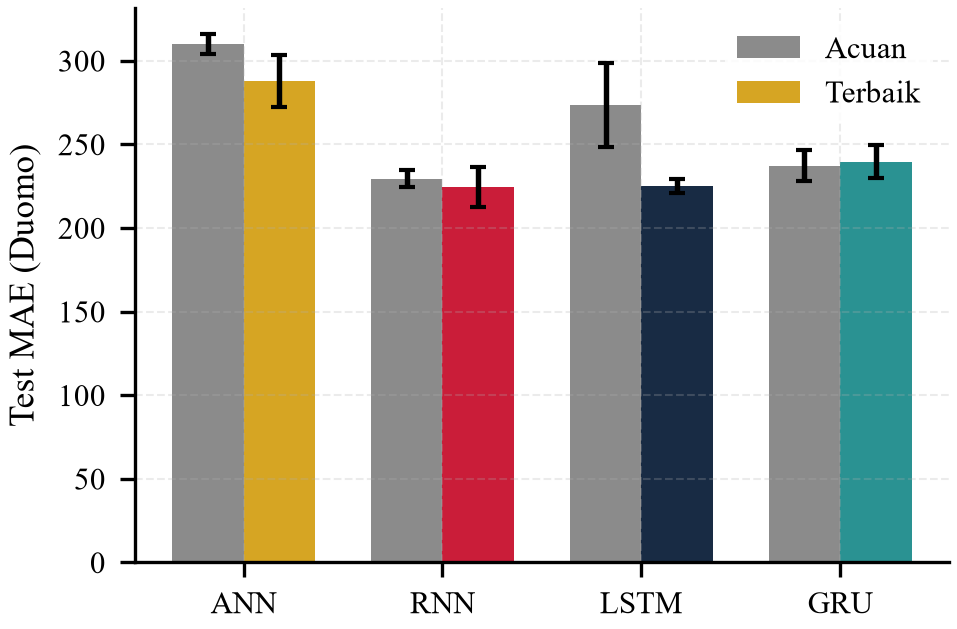
\includegraphics[width=0.9\linewidth]{ieee_col_C_terbaik_vs_acuan.png}
  \caption{Perbandingan Test MAE konfigurasi acuan dan terbaik di Duomo.}
  \label{fig:ieee_col_C_terbaik_vs_acuan}
\end{figure}

Penyetelan gabungan sukses meningkatkan performa uji pada 3 dari 4 model. Test MAE ANN turun dari $309.9$ ke $288.1$, RNN membaik ke $224.5$, dan LSTM melonjak sangat signifikan dari $273.6$ ke $225.3 \pm 4.0$ dengan MAPE paling presisi ($7.3 \pm 0.7\%$). Seluruh model mengungguli baseline naif terbaik ($467.6$) dengan margin $>50\%$. Simple RNN terbaik menjadi model paling tangguh pada periode libur Natal ($404.5 \pm 9.9$). Sebaliknya, konfigurasi terbaik GRU mengalami sedikit degradasi pada data uji ($239.7$ vs acuan $237.2$) akibat pertumbuhan parameter yang melonjak 28 kali lipat (151.809 param) yang memicu \textit{overfitting} validasi.

\subsection{Bagian D — Uji Generalisasi}

Pengujian generalisasi dilakukan pada lokasi kelompok: Navigli (Darsena), kotak 4555 dengan kode lokasi 1 (Tabel~\ref{tab:generalisasi_navigli}, Gambar~\ref{fig:ieee_col_D_generalisasi}, dan Gambar~\ref{fig:D_pola_lokasi}).

\begin{table}[t]
  \centering
  \caption{Uji Generalisasi di Navigli (Kotak 4555, Kode 1, 3 seed)}
  \label{tab:generalisasi_navigli}
  \begin{tabular}{@{}llccccc@{}}
    \toprule
    Model & Konfig. & Param & Val MAE & Test MAE & Test MAPE & Natal MAE \\
    \midrule
    \multirow{2}{*}{ANN} & Acuan & 6,497 & $166.6 \pm 5.3$ & $222.3 \pm 27.4$ & $8.9 \pm 1.1\%$ & $664.5 \pm 190.8$ \\
     & \textbf{Terbaik} & 4,097 & $138.4 \pm 1.7$ & $\mathbf{191.1 \pm 1.9}$ & $\mathbf{7.9 \pm 0.1\%}$ & $607.7 \pm 56.1$ \\
    \midrule
    \multirow{2}{*}{RNN} & Acuan & 5,305 & $147.3 \pm 4.9$ & $\mathbf{193.0 \pm 9.7}$ & $7.8 \pm 0.3\%$ & $534.7 \pm 148.9$ \\
     & Terbaik & 5,305 & $148.7 \pm 7.7$ & $211.7 \pm 24.3$ & $8.7 \pm 1.0\%$ & $649.2 \pm 92.5$ \\
    \midrule
    \multirow{2}{*}{LSTM} & Acuan & 5,578 & $164.3 \pm 9.3$ & $247.3 \pm 54.3$ & $10.0 \pm 2.7\%$ & $950.8 \pm 110.9$ \\
     & \textbf{Terbaik} & 70,273 & $147.2 \pm 4.2$ & $\mathbf{210.4 \pm 7.7}$ & $8.5 \pm 0.5\%$ & $738.4 \pm 41.9$ \\
    \midrule
    \multirow{2}{*}{GRU} & Acuan & 5,397 & $149.0 \pm 6.0$ & $\mathbf{190.8 \pm 6.8}$ & $7.8 \pm 0.2\%$ & $496.4 \pm 50.9$ \\
     & Terbaik & 151,809 & $132.5 \pm 2.1$ & $223.1 \pm 17.0$ & $9.6 \pm 0.7\%$ & $753.7 \pm 49.8$ \\
    \bottomrule
  \end{tabular}
\end{table}

\begin{figure}[t]
  \centering
  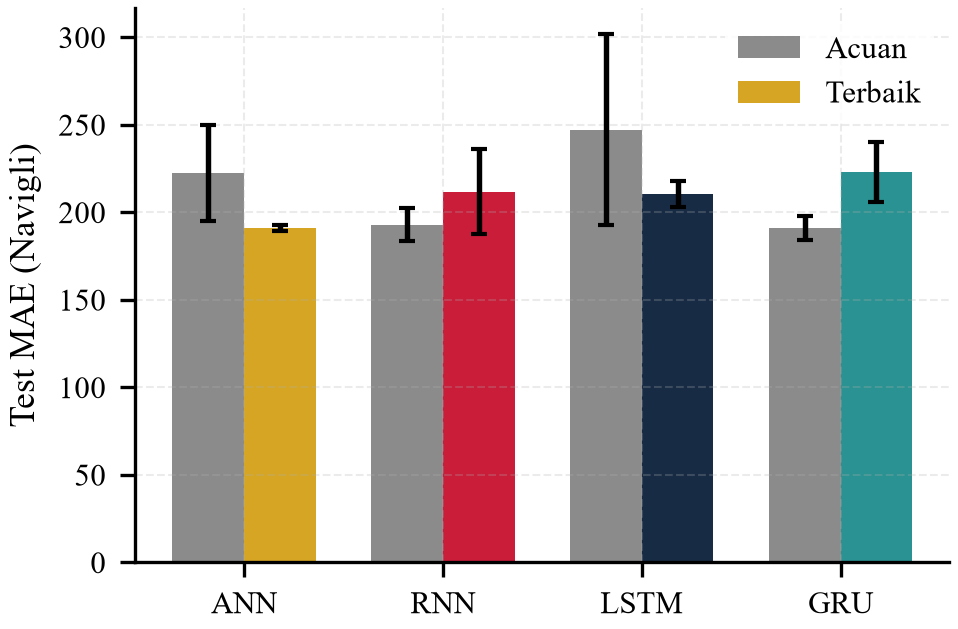
\includegraphics[width=0.9\linewidth]{ieee_col_D_generalisasi.png}
  \caption{Test MAE konfigurasi acuan dan terbaik di Navigli.}
  \label{fig:ieee_col_D_generalisasi}
\end{figure}

\begin{figure}[t]
  \centering
  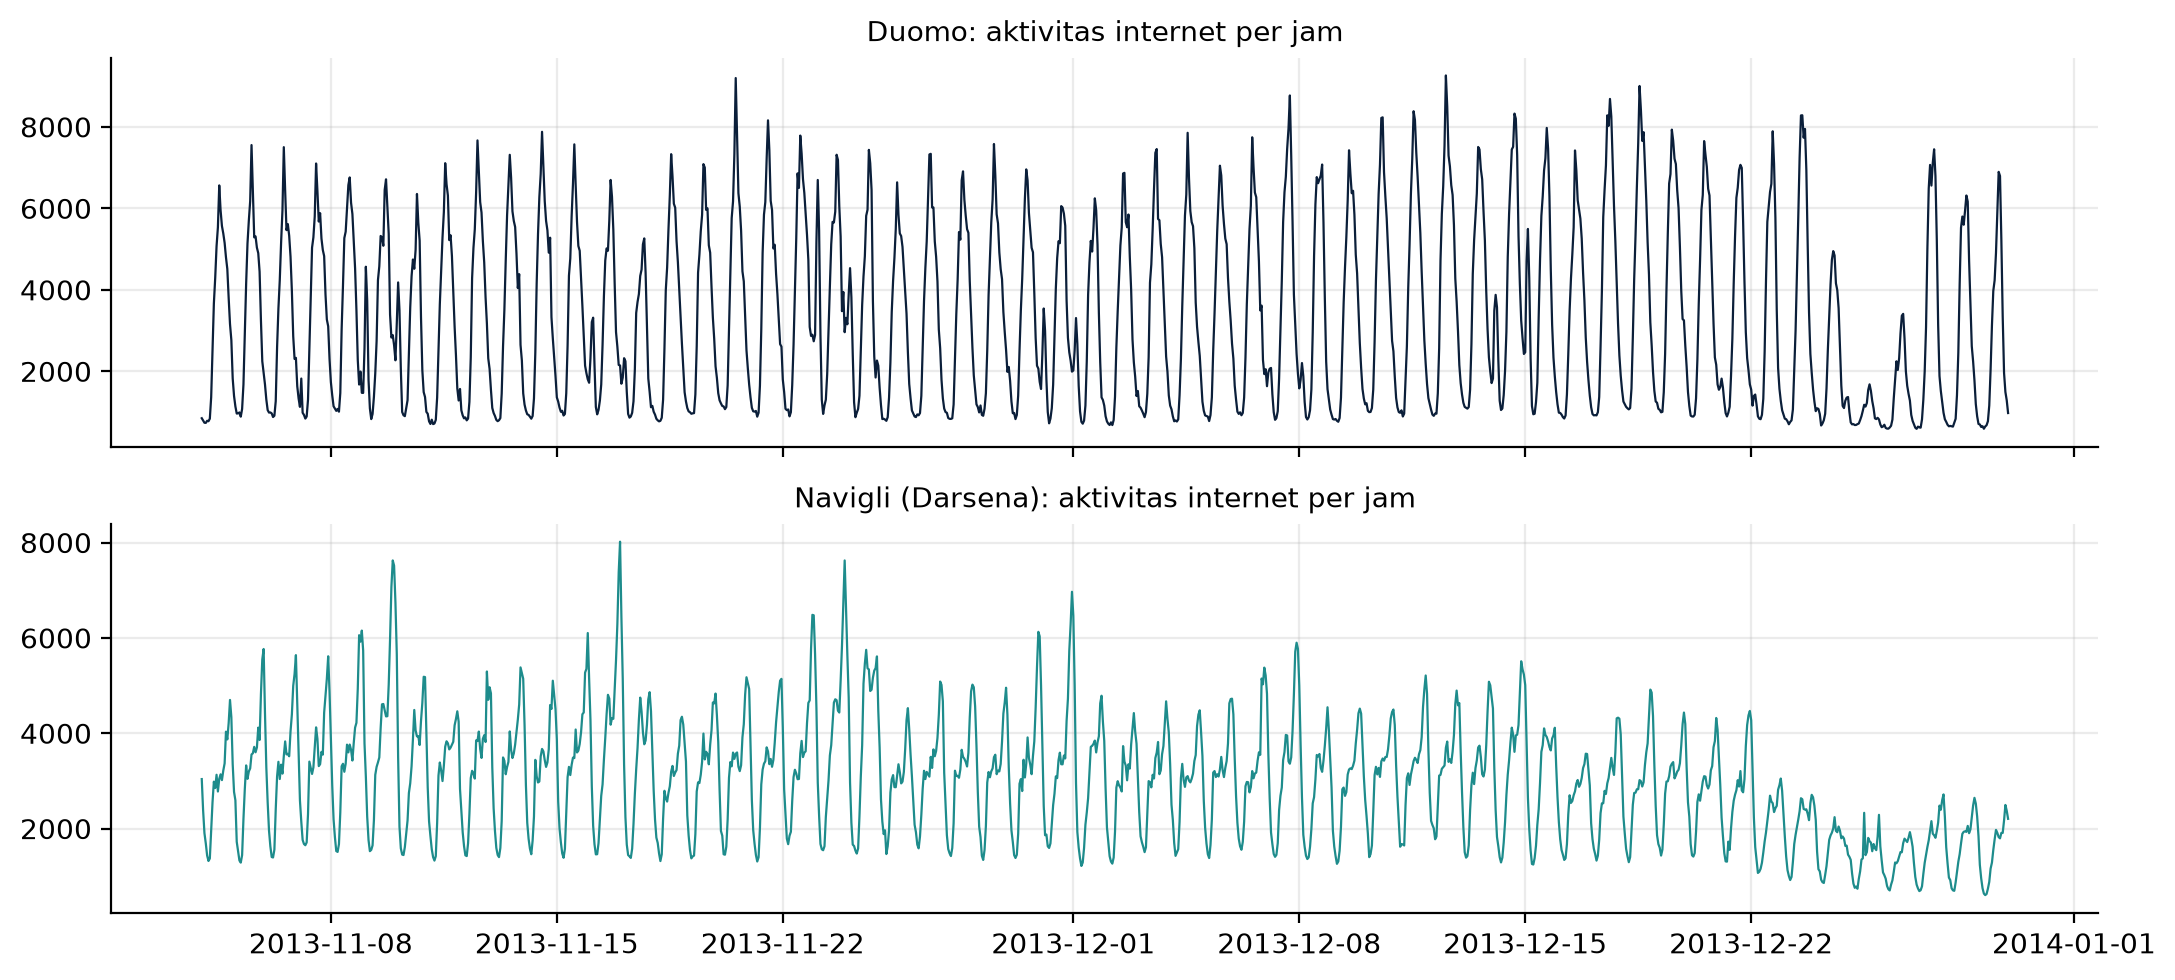
\includegraphics[width=0.9\linewidth]{D_pola_lokasi.png}
  \caption{Perbandingan pola aktivitas internet seluler per jam antara Duomo (kotak 5060) dan Navigli (kotak 4555).}
  \label{fig:D_pola_lokasi}
\end{figure}

\textbf{Pembalikan Peringkat Model:} Evaluasi di Navigli menunjukkan fenomena pergeseran struktural yang dramatis. Di Duomo, model rekuren mendominasi dan ANN selalu berada di posisi terbawah. Sebaliknya di Navigli, konfigurasi terbaik ANN melesat menjadi \textbf{model terbaik nomor satu} ($191.1 \pm 1.9$), mengungguli seluruh model rekuren (LSTM $210.4$, RNN $211.7$, GRU $223.1$).

\textbf{Korelasi dengan Karakter Spasial:} Navigli adalah distrik hiburan malam (\textit{nightlife}) yang dipenuhi kafe dan kanal Darsena. Jika Duomo dicirikan oleh ritme kerja siang hari (Senin--Jumat), Navigli memiliki lonjakan tajam pada malam hingga dini hari (20.00--03.00) dan akhir pekan (Gambar~\ref{fig:D_pola_lokasi}). Jendela pendek ($W=6$ pada ANN dan LSTM) membaca lonjakan instan secara responsif tanpa terdistorsi riwayat 2 hari sebelumnya ($W=48$ pada RNN dan GRU). Ditambah pemetaan deterministik fitur waktu kontinu, ANN meraih akurasi tertinggi dengan variansi paling rapat ($\pm 1.9$).

% ---------------------------------------------------------------------
\section{Pembahasan}

\subsection{Mengapa Hasil Terjadi}
Keunggulan model deep learning dalam peramalan deret waktu seluler bergantung pada kecocokan arsitektur memori dengan dinamika spasial-temporal lokasi. Di kawasan perkantoran teratur seperti Duomo, relasi temporal berulang mingguan secara stasioner, menguntungkan pemrosesan memori sekuensial rekuren. Sebaliknya pada kawasan impulsif seperti Navigli, memori historis panjang ($W=48$) menjadi beban induktif yang merugikan; jaringan feedforward dengan jendela pendek ($W=6$) dan fitur waktu deterministik terbukti jauh lebih adaptif.

\subsection{Faktor Paling dan Paling Tidak Berpengaruh}
Faktor paling berpengaruh meliputi ukuran hidden (A2) dan \textit{learning rate} (A4), yang menentukan transisi dari \textit{severe underfitting} ke saturasi representasi, serta panjang jendela $W$ (A1) yang memicu pelipatgandaan bobot linier pada ANN. Kedalaman layer LSTM (A3) memicu degradasi katastropik pada 3 lapisan akibat \textit{vanishing gradient}. Faktor paling tidak berpengaruh adalah kedalaman ANN (A3, variasi val MAE marjinal antara $240.9$--$248.9$) serta penambahan kanal panggilan dan SMS pada ANN (A5).

\subsection{Variasi Antar-Seed vs Perbedaan Antar-Model}
Di Duomo, margin perbedaan antar-model (acuan RNN $229.6$ vs ANN $309.9$, selisih 80,3) jauh melampaui simpangan baku antar-seed ($\pm 5.1$ hingga $\pm 25.4$), membuktikan keunggulan struktural yang nyata. Namun pada arsitektur berkapasitas raksasa (LSTM acuan $\pm 25.4$, atau Navigli acuan $\pm 54.3$), variansi stokastik melebar, menegaskan pentingnya protokol evaluasi multi-seed untuk integritas ilmiah.

\subsection{Keterbatasan Studi}
Studi ini dibatasi oleh evaluasi dua lokasi seluler di satu kota (Milan) dengan durasi 56 hari (4 minggu data latih). Pembagian waktu kronologis tunggal tanpa validasi bergulir (\textit{walk-forward}) serta ketiadaan variasi hari libur panjang selain minggu Natal menjadi keterbatasan utama generalisasi jangka panjang.

% ---------------------------------------------------------------------
\section{Kesimpulan}

Studi ablasi terkontrol ini membuktikan bahwa pada kawasan perkantoran Duomo (Milan), model sekuensial rekuren secara konsisten mengungguli feedforward ANN dan baseline naif, di mana Simple RNN acuan mencatat test MAE $229.6 \pm 5.1$ dibandingkan ANN $309.9 \pm 5.9$ dan naif minggu lalu $467.6$. Penyetelan konfigurasi berbasis val MAE berhasil meningkatkan akurasi LSTM menjadi $225.3 \pm 4.0$ (MAPE terbaik $7.3\%$) dan RNN menjadi $224.5 \pm 11.7$, namun arsitektur berkapasitas berlebih seperti GRU terbaik (151.809 parameter) mengalami overfitting yang mendegradasi performa uji menjadi $239.7 \pm 9.9$. Uji generalisasi di kawasan hiburan malam Navigli membalikkan urutan model secara total, di mana model ANN terbaik dengan jendela pendek ($W=6$) melesat menjadi model nomor satu (test MAE $191.1 \pm 1.9$). Temuan ini menegaskan bahwa efektivitas arsitektur deep learning sangat terikat pada pola spasial-temporal lokal dan seleksi hyperparameter murni berbasis validasi membutuhkan kontrol regularisasi yang ketat.

% ---------------------------------------------------------------------
\section*{Kontribusi Anggota}
\begin{tabular}{@{}lp{0.62\linewidth}@{}}
  Adif Dafa Raihan & Penyusunan kode eksperimen dasar, penulisan Pendahuluan, Data dan Metode, konfigurasi acuan, serta protokol evaluasi. \\
  Cindy Auliya & Eksekusi eksperimen ablasi wajib A1--A5 dan pilihan B2/B6, visualisasi grafik IEEE, serta penulisan Bagian 0, A, dan B. \\
  Bima Cahya Ramadhan & Eksekusi konfigurasi terbaik (Bagian C), uji generalisasi Navigli (Bagian D), penulisan Pembahasan, dan penyusunan Kesimpulan akhir. \\
\end{tabular}

\section*{Pernyataan Penggunaan AI}
Kami menggunakan bantuan asisten AI, antara lain OpenCode, untuk membantu penulisan kode eksperimen, analisis awal, dan penyuntingan bahasa laporan. Seluruh rancangan eksperimen, eksekusi pelatihan, dan angka yang dilaporkan berasal dari run kelompok sendiri yang tersimpan pada \texttt{hasil/ablasi.csv}; setiap keluaran AI diperiksa ulang terhadap data tersebut. AI tidak dipakai untuk memanipulasi angka hasil.

\section*{Kode dan Data}
Kode, notebook beserta output, dan seluruh hasil run tersedia di \url{https://github.com/dapaaap/milan-traffic-ablation-01}.

\bibliographystyle{IEEEtran}
\bibliography{references}

\end{document}
